% You should title the file with a .tex extension (hw1.tex, for example)
\documentclass[11pt]{article}

\usepackage{amsmath}
\usepackage{amssymb}
\usepackage{fancyhdr}
\usepackage{hyperref}
\usepackage{graphicx}

\oddsidemargin0cm
\topmargin-2cm     %I recommend adding these three lines to increase the 
\textwidth16.5cm   %amount of usable space on the page (and save trees)
\textheight23.5cm  

\newcommand{\question}[2] {\vspace{.25in} \hrule\vspace{0.5em}
\noindent{\bf #1: #2} \vspace{0.5em}
\hrule \vspace{.10in}}
\renewcommand{\part}[1] {\vspace{.10in} {\bf (#1)}}

\newcommand{\myname}{Charles Liu}
\newcommand{\myandrew}{cliu02@g.harvard.edu}
\newcommand{\myhwnum}{1}

\pagestyle{fancyplain}
\lhead{\fancyplain{}{\textbf{HW\myhwnum}}}      % Note the different brackets!
\rhead{\fancyplain{}{\myname\\ \myandrew}}
\chead{\fancyplain{}{CS284}}

\begin{document}

\medskip                        % Skip a "medium" amount of space
                                % (latex determines what medium is)
                                % Also try: \bigskip, \littleskip

\thispagestyle{plain}
\begin{center}                  % Center the following lines
{\Large CS284 Problem Set \myhwnum} \\
\myname \\
\myandrew \\
\today\\
\end{center}

\question{1}{Install Drake}
Had one issue with vtk5 --with-qt brew package, but workaround found here: \url{https://github.com/RobotLocomotion/drake/issues/1673}

\question{2}{Fully-actuated definition}
False: You can have the number of actuators equal the number of degrees of freedom and still have an underactuated system. In the example of the affine system $\ddot{q} = f_1(q, \dot{q}, t) + f_2(q,\dot{q},t)u$, there was a necessary condition of $rank[f_2(q,\dot{q},t)] = dim[q]$ for the system to be fully actuated. There could be holonomic constraints that limit the range of inputs over the actuators that would essentially reduce one degree of freedom and cause an underactuated system as well.

\question{3}{Underactuated systems}
\part{a}
The system has 3 degrees of freedom ($x$,$z$,$\theta$) but only two actuators so the system must be underactuated.

\part{b}
The system again has 3 degrees of freedom ($x$,$y$,$\theta$) whereas you can only maneuver with $f$ and $\alpha$ so the system is underactuated.

\part{c}
If nonholonomic systems have constraints on velocity, you can take the derivative over time and get a constraint on acceleration. By definition that's an underactuated system.

\part{d}

i. Define $p_3$ to be the point $l_1$ from the foot, and $p_4$ to be the point $l2$ from $p_3$. The [x,y] vectors for these points are:
\begin{eqnarray*}
	p_1 &=& [x-dcos(\theta),y-dsin(\theta)]\\
	p_2 &=& [x+dcos(\theta),y+dsin(\theta)]\\
	p_3 &=& [x+l_1sin(\alpha_1), y+l_1cos(\alpha_1)]\\
	p_4 &=& p_3 + [-l_2sin(\alpha_2-\alpha_1), l_2cos(\alpha_2-\alpha_1)]
\end{eqnarray*}

The values for $p_4$ are obtained by forming a triangle between $l_1,l_2$ and an imaginary line from the second pendulum point to the center. The angle we are looking for, $x$, is formed by the imaginary line and $l_2$. As $\alpha_2$ and the angle between $l_1$ and $l_2$ form a line, we have the equation $180-x-\alpha_1+\alpha_2 = 180$, which gives us $x=\alpha_2-\alpha_1$. The derivatives are then:
\begin{eqnarray*}
	\dot{p_1} &=& [\dot{x}+dsin(\theta),\dot{y}-dcos(\theta)]\\
	\dot{p_2} &=& [\dot{x}-dsin(\theta),\dot{y}+dcos(\theta)]\\
	\dot{p_3} &=& [\dot{x} + l_1\dot{\alpha_1}cos(\alpha_1), \dot{y}-l_1\dot{\alpha_1}sin(\alpha_1)]\\
	\dot{p_4} &=& \dot{p_3} + [l_2cos(\alpha_2-\alpha_1)(\dot{\alpha_1} - \dot{\alpha_2}), l_2sin(\alpha_2-\alpha_1)(\dot{\alpha_1}-\dot{\alpha_2})]
\end{eqnarray*}

The equations for energy are then (using identities $sin^2+cos^2=1$, $cos(a-b)=cosacosb+sinasinb$, $sin(a-b)=sinacosb-cosasinb$:
\begin{eqnarray*}
	T &=& \frac{1}{2}(m_1\dot{p_1}\dot{p_1}^T + m_2\dot{p_2}\dot{p_2}^T + m_3\dot{p_3}\dot{p_3}^T + m_4\dot{p_4}\dot{p_4}^T)\\
	  &=& \frac{1}{2}(\sum m_i)(\dot{x}^2+\dot{y}^2) + \frac{1}{2}(m_1+m_2)d^2 + \frac{1}{2}(m_1-m_2)(2dsin(\theta)-2dcos(\theta)) +\\
	  && \frac{1}{2}(m_3+m_4)(l_1^2\dot{\alpha_1}^2)-(m_3+m_4)(\dot{x}l_1\dot{\alpha_1}cos(\alpha_1)-\dot{y}l_1\dot{\alpha_1}sin(\alpha_1)) +\\
	  && \frac{1}{2}m_4(\dot{\alpha_1}-\dot{\alpha_2})(l_2^2(\dot{\alpha_1}-\dot{\alpha_2}) + 2l_1l_2\dot{\alpha_1}cos(\alpha_2) + \dot{y}l_2sin(\alpha_2-\alpha_1))\\
	U &=& (m_3+m_4)gl_1cos(\alpha_1) + m_4gl_2(cos(\alpha_1)cos(\alpha_2) + sin(\alpha_1)sin(\alpha_2))\\
	L &=& T-U\\
	  &=& \frac{1}{2}(\sum m_i)(\dot{x}^2+\dot{y}^2) + \frac{1}{2}(m_1+m_2)d^2 + \frac{1}{2}(m_1-m_2)(2dsin(\theta)-2dcos(\theta)) +\\
	  && \frac{1}{2}(m_3+m_4)(l_1^2\dot{\alpha_1}^2)-(m_3+m_4)(\dot{x}l_1\dot{\alpha_1}cos(\alpha_1)-\dot{y}l_1\dot{\alpha_1}sin(\alpha_1)) +\\
	  && \frac{1}{2}m_4(\dot{\alpha_1}-\dot{\alpha_2})(l_2^2(\dot{\alpha_1}-\dot{\alpha_2}) + 2l_1l_2\dot{\alpha_1}cos(\alpha_2) + \dot{y}l_2sin(\alpha_2-\alpha_1))- \\
	  && (m_3+m_4)gl_1cos(\alpha_1) + m_4gl_2(cos(\alpha_1)cos(\alpha_2) + sin(\alpha_1)sin(\alpha_2))
\end{eqnarray*}

Define the input vector $u$ to be of the form $[f_{1x},f_{1y},f_{2x},f_{2y},\tau_1,\tau_2]^T$ where $f_{ij}$ is the force component of $f_i$ on direction $j$. Using the Lagrangian we get:

\begin{eqnarray*}
	f_{1x}+f_{2x} &=& Q_{\dot{x}} = \frac{1}{2}(\sum m_i)\ddot{x} + (m_3+m_4)(l_1\ddot{\alpha_1}cos(\alpha_1) - l_1\dot{\alpha_1}^2sin(\alpha_1))\\
	f_{1y}+f_{2y} &=& Q_{\dot{y}} ...\\
	f_{1x}+f_{1y}+f_{2x}+f{2y} &=& ...\\
	\tau_1 &=& ...\\
	\tau_2 &=& ...\\
\end{eqnarray*}

I'm sure this is wrong, especially because $p_3$ and $p_4$ aren't accounting for $\theta$ which it should but can't figure out how the geometry works out. I think it will be an underactuated system in this case because for the input vector $u$, the matrix $\mathbb{B}$ will be of the form:

\[ \left| \begin{array}{cccccc}
	1 & 0 & 1 & 0 & 0 & 0 \\
	0 & 1 & 0 & 1 & 0 & 0 \\
	1 & 1 & 1 & 1 & 0 & 0 \\
	0 & 0 & 0 & 0 & 1 & 0 \\
	0 & 0 & 0 & 0 & 0 & 1
	\end{array} \right| \]

where the third row ($\theta$) is some linear combination on the first two ($x$ and $y$) and does not satisfy the rank condition.

ii. When in the air there are no $f_1$,$f_2$ components so the number of actuators is only $\tau_1$,$\tau_2$ which is underactuated for the $q$ configuration.

\question{4}{Feedback Linearization}
False: Although any $\ddot{q}$ can be achieved by setting $u=B^{-1}[C(q,\dot{q}) + H(q)\ddot{q}_{des}]$, the same cannot be said for $\dot{q}$ as the function $C(q,\dot{q})$ may not easily be decoupled.

\question{5}{Pendulum dynamics}
\part{a} 
This can be described by the following:

\[ \dot{x} = \left| \begin{array}{c}
	\dot{\theta} \\
	 -\dot{\theta} - 10sin\theta - 5\end{array} \right| \] 

Fixed points are $\frac{-5\pi}{6}$ and $\frac{-\pi}{6}$ with $\dot{\theta}=0$. The Jacobian matrix is:
\[ \left| \begin{array}{cc}
	0 & 1 \\
	-10cos\theta & -1 \end{array} \right| \]

The eigenvalues for this matrix are $\frac{-1 +/- \sqrt{1-40cos\theta}}{2}$. In the case of $-\frac{\pi}{6}$ these are complex eigenvalues with a negative real component so it is a stable fixed point. In the case of $-\frac{5\pi}{6}$ there's one positive eigenvalue and one negative, so this is an unstable point. Source: \url{https://controls.engin.umich.edu/wiki/index.php/EigenvalueStability}

\part{b} In the case of $\ddot{\theta} = -\dot{\theta} - 10sin\theta + 10$ the only fixed point is $\theta = \frac{\pi}{2}, \dot{\theta} = 0$ which is unstable as its eigenvalues are 0 and -1. If $u>10$ there are no fixed points.

\question{6}{Graphical Analysis}
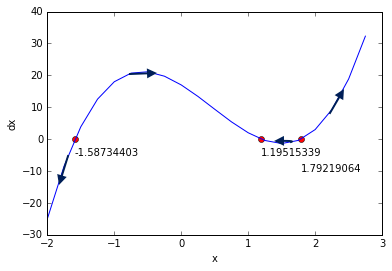
\includegraphics{q6}

The only stable point is at 1.19515339, the others are unstable.

\question{7}{Lyapunov Analysis}
\begin{eqnarray*}
	V &=& \frac{1}{2}x^Tx = \frac{x_1^2+x_2^2}{2} \\
	\dot{x_1} &=& -x_2-x_1(1-x_1^2-x_2^2) \\
	\dot{x_2} &=& x_1-x_2(1-x_1^2-x_2^2) \\
	\dot{V} &=& x_1\dot{x_1} + x_2\dot{x_2} \\
			&=& x_1(-x_2-x_1(1-x_1^2-x_2^2)) + x_2(x_1-x_2(1-x_1^2-x_2^2))\\
			&=& -x_1x_2 - x_1^2(1-x_1^2-x_2^2) + x_1x_2-x_2^2(1-x_1^2-x_2^2)\\
			&=& -(x_1^2+x_2^2)(1-x_1^2-x_2^2) \\
			&=& -(x_1^2+x_2^2)(1-(x_1^2+x_2^2))
\end{eqnarray*}

V is clearly always positive with non-zero $x_1,x_2$. $\dot{V} < 0$ if $x_1^2+x_2^2 < 1$, so it is locally asymptotically stable as there is a bounded region where it is negative. However, once $x_1^2+x_2^2 > 0$, then the value is positive so it is not globally stable.

\question{8}{Discrete Time Systems}
\part{a}
\begin{eqnarray*}
	f(x)   &=& -x\\
	x[k+1] &=& x[k] - hx[k]\\
		   &=& x[k](1 - h)
\end{eqnarray*}
For $0<h<1$, the value of $x[k]$ will converge to $x^*=0$, but if $h>1$ $x[k]$ will just keep growing in absolute value.

\part{b}
As implied previously, $h^*=1$ so $h^*=g$

\question{9}{Lecture survey}
\part{b} Not having taken a physics class since high school, the mechanics stuff is totally new for me so it was a bit fast, but I don't think any pace would have been slow enough given this isn't a mechanics course so you can't spend too much time on it.

\question{10}{Problem set survey}
About 10 hours

\question{11}{Your background}
Graduated in 2011 studying CS/Financial Engineering, worked in finance for the last 4 years.


\end{document}

